% Created 2020-08-28 周五 19:04
% Intended LaTeX compiler: pdflatex
\documentclass[11pt]{article}
\usepackage[utf8]{inputenc}
\usepackage[T1]{fontenc}
\usepackage{graphicx}
\usepackage{grffile}
\usepackage{longtable}
\usepackage{wrapfig}
\usepackage{rotating}
\usepackage[normalem]{ulem}
\usepackage{amsmath}
\usepackage{textcomp}
\usepackage{amssymb}
\usepackage{capt-of}
\usepackage{hyperref}
\usepackage{minted}
%%%%%%%%%%%%%%%%%%%%%%%%%%%%%%%%%%%%%%
%% TIPS                                 %%
%%%%%%%%%%%%%%%%%%%%%%%%%%%%%%%%%%%%%%
% \substack{a\\b} for multiple lines text

\usepackage[utf8]{inputenc}

\usepackage[B1,T1]{fontenc}

% pdfplots will load xolor automatically without option
\usepackage[dvipsnames]{xcolor}
%%%%%%%%%%%%%%%%%%%%%%%%%%%%%%%%%%%%%%%
%% MATH related pacakge                  %%
%%%%%%%%%%%%%%%%%%%%%%%%%%%%%%%%%%%%%%%
% \usepackage{amsmath} mathtools loads the amsmath
\usepackage{amsmath}
\usepackage{mathtools}


\usepackage{amsthm}
\usepackage{amsbsy}

%\usepackage{commath}

\usepackage{amssymb}
\usepackage{mathrsfs}
%\usepackage{mathabx}
\usepackage{stmaryrd}
\usepackage{empheq}

\usepackage{scalerel}
\usepackage{stackengine}
\usepackage{stackrel}

\usepackage{nicematrix}
\usepackage{tensor}
\usepackage{blkarray}
\usepackage{siunitx}
\usepackage[f]{esvect}

\usepackage{unicode-math}
\setmainfont{TeX Gyre Pagella}
% \setmathfont{STIX}
% \setmathfont{texgyrepagella-math.otf}
% \setmathfont{Libertinus Math}
\setmathfont{Latin Modern Math}
\setmathfont[range={\mscra,\mscrb,\mscrc,\mscrd,\mscre,\mscrf,\mscrg,\mscrh,\mscri,\mscrj,\mscrk,\mscrl,\mscrm,\mscrn,\mscro,\mscrp,\mscrq,\mscrr,\mscrs,\mscrt,\mscru,\mscrv,\mscrw,\mscrx,\mscry,\mscrz,\mscrA,\mscrB,\mscrC,\mscrD,\mscrE,\mscrF,\mscrG,\mscrH,\mscrI,\mscrJ,\mscrK,\mscrL,\mscrM,\mscrN,\mscrO,\mscrP,\mscrQ,\mscrR,\mscrS,\mscrT,\mscrU,\mscrV,\mscrW,\mscrX,\mscrY,\mscrZ}]{Latin Modern Math}
\setmathfont[range={\smwhtdiamond,\enclosediamond,\varlrtriangle}]{Latin Modern Math}
\setmathfont[range={\rightrightarrows,\twoheadrightarrow,\leftrightsquigarrow,\triangledown}]{XITS Math}
\setmathfont[range={\int,\setminus}]{Libertinus Math}



%%%%%%%%%%%%%%%%%%%%%%%%%%%%%%%%%%%%%%%
%% TIKZ related packages                 %%
%%%%%%%%%%%%%%%%%%%%%%%%%%%%%%%%%%%%%%%

\usepackage{pgfplots}
\pgfplotsset{compat=1.15}
\usepackage{tikz}
\usepackage{tikz-cd}
\usepackage{tikz-qtree}

\usetikzlibrary{arrows,positioning,calc,fadings,decorations,matrix,decorations,shapes.misc}
%setting from geogebra
\definecolor{ccqqqq}{rgb}{0.8,0,0}


%%%%%%%%%%%%%%%%%%%%%%%%%%%%%%%%%%%%%%%
%% MISCLELLANEOUS packages               %%
%%%%%%%%%%%%%%%%%%%%%%%%%%%%%%%%%%%%%%%
\usepackage[most]{tcolorbox}
\usepackage{threeparttable}
\usepackage{tabularx}

\usepackage{enumitem}

% wrong with preview
\usepackage{subcaption}
\usepackage{caption}
% {\aunclfamily\Huge}
\usepackage{auncial}

\usepackage{float}

\usepackage{fancyhdr}

\usepackage{ifthen}
\usepackage{xargs}


\usepackage{imakeidx}
\usepackage{hyperref}
\usepackage{soul}


%\usepackage[xetex]{preview}
%%%%%%%%%%%%%%%%%%%%%%%%%%%%%%%%%%%%%%%
%% USEPACKAGES end                       %%
%%%%%%%%%%%%%%%%%%%%%%%%%%%%%%%%%%%%%%%

% \setlist{nosep}
% \numberwithin{equation}{subsection}
% \fancyhead{} % Clear the headers
% \renewcommand{\headrulewidth}{0pt} % Width of line at top of page
% \fancyhead[R]{\slshape\leftmark} % Mark right [R] of page with Chapter name [\leftmark]
% \pagestyle{fancy} % Set default style for all content pages (not TOC, etc)


% \newlength\shlength
% \newcommand\vect[2][0]{\setlength\shlength{#1pt}%
%   \stackengine{-5.6pt}{$#2$}{\smash{$\kern\shlength%
%     \stackengine{7.55pt}{$\mathchar"017E$}%
%       {\rule{\widthof{$#2$}}{.57pt}\kern.4pt}{O}{r}{F}{F}{L}\kern-\shlength$}}%
%       {O}{c}{F}{T}{S}}


\indexsetup{othercode=\small}
\makeindex[columns=2,options={-s /media/wu/file/stuuudy/notes/index_style.ist},intoc]
\makeatletter
\def\@idxitem{\par\hangindent 0pt}
\makeatother


%\newcounter{dummy} \numberwithin{dummy}{section}
\newtheorem{dummy}{dummy}[section]
\theoremstyle{definition}
\newtheorem{definition}[dummy]{Definition}
\theoremstyle{plain}
\newtheorem{corollary}[dummy]{Corollary}
\newtheorem{lemma}[dummy]{Lemma}
\newtheorem{proposition}[dummy]{Proposition}
\newtheorem{theorem}[dummy]{Theorem}
\theoremstyle{definition}
\newtheorem{examplle}{Example}[section]
\theoremstyle{remark}
\newtheorem*{remark}{Remark}
\newtheorem{exercise}{Exercise}[subsection]
\newtheorem{observation}{Observation}[section]


\newenvironment{claim}[1]{\par\noindent\textbf{Claim:}\space#1}{}

\makeatletter
\DeclareFontFamily{U}{tipa}{}
\DeclareFontShape{U}{tipa}{m}{n}{<->tipa10}{}
\newcommand{\arc@char}{{\usefont{U}{tipa}{m}{n}\symbol{62}}}%

\newcommand{\arc}[1]{\mathpalette\arc@arc{#1}}

\newcommand{\arc@arc}[2]{%
  \sbox0{$\m@th#1#2$}%
  \vbox{
    \hbox{\resizebox{\wd0}{\height}{\arc@char}}
    \nointerlineskip
    \box0
  }%
}
\makeatother

\setcounter{MaxMatrixCols}{20}
%%%%%%% ABS
\DeclarePairedDelimiter\abss{\lvert}{\rvert}%
\DeclarePairedDelimiter\normm{\lVert}{\rVert}%

% Swap the definition of \abs* and \norm*, so that \abs
% and \norm resizes the size of the brackets, and the
% starred version does not.
\makeatletter
\let\oldabs\abss
%\def\abs{\@ifstar{\oldabs}{\oldabs*}}
\newcommand{\abs}{\@ifstar{\oldabs}{\oldabs*}}
\newcommand{\norm}[1]{\left\lVert#1\right\rVert}
%\let\oldnorm\normm
%\def\norm{\@ifstar{\oldnorm}{\oldnorm*}}
%\renewcommand{norm}{\@ifstar{\oldnorm}{\oldnorm*}}
\makeatother

% \newcommand\what[1]{\ThisStyle{%
%     \setbox0=\hbox{$\SavedStyle#1$}%
%     \stackengine{-1.0\ht0+.5pt}{$\SavedStyle#1$}{%
%       \stretchto{\scaleto{\SavedStyle\mkern.15mu\char'136}{2.6\wd0}}{1.4\ht0}%
%     }{O}{c}{F}{T}{S}%
%   }
% }

% \newcommand\wtilde[1]{\ThisStyle{%
%     \setbox0=\hbox{$\SavedStyle#1$}%
%     \stackengine{-.1\LMpt}{$\SavedStyle#1$}{%
%       \stretchto{\scaleto{\SavedStyle\mkern.2mu\AC}{.5150\wd0}}{.6\ht0}%
%     }{O}{c}{F}{T}{S}%
%   }
% }

% \newcommand\wbar[1]{\ThisStyle{%
%     \setbox0=\hbox{$\SavedStyle#1$}%
%     \stackengine{.5pt+\LMpt}{$\SavedStyle#1$}{%
%       \rule{\wd0}{\dimexpr.3\LMpt+.3pt}%
%     }{O}{c}{F}{T}{S}%
%   }
% }

\newcommand{\bl}[1] {\boldsymbol{#1}}
\newcommand{\Wt}[1] {\stackrel{\sim}{\smash{#1}\rule{0pt}{1.1ex}}}
\newcommand{\wt}[1] {\widetilde{#1}}
\newcommand{\tf}[1] {\textbf{#1}}


%For boxed texts in align, use Aboxed{}
%otherwise use boxed{}

\DeclareMathSymbol{\widehatsym}{\mathord}{largesymbols}{"62}
\newcommand\lowerwidehatsym{%
  \text{\smash{\raisebox{-1.3ex}{%
    $\widehatsym$}}}}
\newcommand\fixwidehat[1]{%
  \mathchoice
    {\accentset{\displaystyle\lowerwidehatsym}{#1}}
    {\accentset{\textstyle\lowerwidehatsym}{#1}}
    {\accentset{\scriptstyle\lowerwidehatsym}{#1}}
    {\accentset{\scriptscriptstyle\lowerwidehatsym}{#1}}
  }


\newcommand{\cupdot}{\mathbin{\dot{\cup}}}
\newcommand{\bigcupdot}{\mathop{\dot{\bigcup}}}

\usepackage{graphicx}

\usepackage[toc,page]{appendix}

% text on arrow for xRightarrow
\makeatletter
%\newcommand{\xRightarrow}[2][]{\ext@arrow 0359\Rightarrowfill@{#1}{#2}}
\makeatother

% Arbitrary long arrow
\newcommand{\Rarrow}[1]{%
\parbox{#1}{\tikz{\draw[->](0,0)--(#1,0);}}
}

\newcommand{\LRarrow}[1]{%
\parbox{#1}{\tikz{\draw[<->](0,0)--(#1,0);}}
}


\makeatletter
\providecommand*{\rmodels}{%
  \mathrel{%
    \mathpalette\@rmodels\models
  }%
}
\newcommand*{\@rmodels}[2]{%
  \reflectbox{$\m@th#1#2$}%
}
\makeatother







\newcommand{\trcl}[1]{%
  \mathrm{trcl}{(#1)}
}



% Roman numerals
\makeatletter
\newcommand*{\rom}[1]{\expandafter\@slowromancap\romannumeral #1@}
\makeatother
% \\def \\b\([a-zA-Z]\) {\\boldsymbol{[a-zA-z]}}
% \\DeclareMathOperator{\\b\1}{\\textbf{\1}}


\DeclareMathOperator{\bx}{\textbf{x}}
\DeclareMathOperator{\bz}{\textbf{z}}
\DeclareMathOperator{\bff}{\textbf{f}}
\DeclareMathOperator{\ba}{\textbf{a}}
\DeclareMathOperator{\bk}{\textbf{k}}
\DeclareMathOperator{\bs}{\textbf{s}}
\DeclareMathOperator{\bh}{\textbf{h}}
\DeclareMathOperator{\bc}{\textbf{c}}
\DeclareMathOperator{\br}{\textbf{r}}
\DeclareMathOperator{\bi}{\textbf{i}}
\DeclareMathOperator{\bj}{\textbf{j}}
\DeclareMathOperator{\bn}{\textbf{n}}
\DeclareMathOperator{\be}{\textbf{e}}
\DeclareMathOperator{\bo}{\textbf{o}}
\DeclareMathOperator{\bU}{\textbf{U}}
\DeclareMathOperator{\bL}{\textbf{L}}
\DeclareMathOperator{\bV}{\textbf{V}}
\def \bzero {\mathbf{0}}
\def \btwo {\mathbf{2}}
\DeclareMathOperator{\bv}{\textbf{v}}
\DeclareMathOperator{\bp}{\textbf{p}}
\DeclareMathOperator{\bI}{\textbf{I}}
\DeclareMathOperator{\bM}{\textbf{M}}
\DeclareMathOperator{\bN}{\textbf{N}}
\DeclareMathOperator{\bK}{\textbf{K}}
\DeclareMathOperator{\bt}{\textbf{t}}
\DeclareMathOperator{\bb}{\textbf{b}}
\DeclareMathOperator{\bA}{\textbf{A}}
\DeclareMathOperator{\bX}{\textbf{X}}
\DeclareMathOperator{\bu}{\textbf{u}}
\DeclareMathOperator{\bS}{\textbf{S}}
\DeclareMathOperator{\bZ}{\textbf{Z}}
\DeclareMathOperator{\by}{\textbf{y}}
\DeclareMathOperator{\bw}{\textbf{w}}
\DeclareMathOperator{\bT}{\textbf{T}}
\DeclareMathOperator{\bF}{\textbf{F}}
\DeclareMathOperator{\bmm}{\textbf{m}}
\DeclareMathOperator{\bW}{\textbf{W}}
\DeclareMathOperator{\bR}{\textbf{R}}
\DeclareMathOperator{\bC}{\textbf{C}}
\DeclareMathOperator{\bD}{\textbf{D}}
\DeclareMathOperator{\bE}{\textbf{E}}
\DeclareMathOperator{\bQ}{\textbf{Q}}
\DeclareMathOperator{\bP}{\textbf{P}}
\DeclareMathOperator{\bY}{\textbf{Y}}
\DeclareMathOperator{\bH}{\textbf{H}}
\DeclareMathOperator{\bB}{\textbf{B}}
\DeclareMathOperator{\bG}{\textbf{G}}
\def \blambda {\symbf{\lambda}}
\def \boldeta {\symbf{\eta}}
\def \balpha {\symbf{\alpha}}
\def \bbeta {\symbf{\beta}}
\def \bgamma {\symbf{\gamma}}
\def \bxi {\symbf{\xi}}
\def \bLambda {\symbf{\Lambda}}

\newcommand{\bto}{{\boldsymbol{\to}}}
\newcommand{\Ra}{\Rightarrow}
\newcommand\und[1]{\underline{#1}}
\def \bPhi {\boldsymbol{\Phi}}
\def \btheta {\boldsymbol{\theta}}
\def \bTheta {\boldsymbol{\Theta}}
\def \bmu {\boldsymbol{\mu}}
\def \bphi {\boldsymbol{\phi}}
\def \bSigma {\boldsymbol{\Sigma}}
\def \lb {\left\{}
\def \rb {\right\}}
\def \la {\langle}
\def \ra {\rangle}
\def \caln {\mathcal{N}}
\def \dissum {\displaystyle\Sigma}
\def \dispro {\displaystyle\prod}
\def \E {\mathbb{E}}
\def \Q {\mathbb{Q}}
\def \N {\mathbb{N}}
\def \V {\mathbb{V}}
\def \R {\mathbb{R}}
\def \P {\mathbb{P}}
\def \A {\mathbb{A}}
\def \F {\mathbb{F}}
\def \Z {\mathbb{Z}}
\def \I {\mathbb{I}}
\def \C {\mathbb{C}}
\def \cala {\mathcal{A}}
\def \cale {\mathcal{E}}
\def \calb {\mathcal{B}}
\def \calq {\mathcal{Q}}
\def \calp {\mathcal{P}}
\def \cals {\mathcal{S}}
\def \calx {\mathcal{X}}
\def \caly {\mathcal{Y}}
\def \calg {\mathcal{G}}
\def \cald {\mathcal{D}}
\def \caln {\mathcal{N}}
\def \calr {\mathcal{R}}
\def \calt {\mathcal{T}}
\def \calm {\mathcal{M}}
\def \calw {\mathcal{W}}
\def \calc {\mathcal{C}}
\def \calv {\mathcal{V}}
\def \calf {\mathcal{F}}
\def \calk {\mathcal{K}}
\def \call {\mathcal{L}}
\def \calu {\mathcal{U}}
\def \calo {\mathcal{O}}
\def \calh {\mathcal{H}}
\def \cali {\mathcal{I}}

\def \bcup {\bigcup}

% set theory

\def \zfcc {\textbf{ZFC}^-}
\def \ac  {\textbf{AC}}
\def \gl  {\textbf{L }}
\def \gll {\textbf{L}}
\newcommand{\zfm}{$\textbf{ZF}^-$}

%\def \zfm {$\textbf{ZF}^-$}
\def \zfmm {\textbf{ZF}^-}
\def \wf {\textbf{WF }}
\def \on {\textbf{On }}
\def \cm {\textbf{M }}
\def \cn {\textbf{N }}
\def \cv {\textbf{V }}
\def \zc {\textbf{ZC }}
\def \zcm {\textbf{ZC}}
\def \zff {\textbf{ZF}}
\def \wfm {\textbf{WF}}
\def \onm {\textbf{On}}
\def \cmm {\textbf{M}}
\def \cnm {\textbf{N}}
\def \cvm {\textbf{V}}
\def \gchh {\textbf{GCH}}
\renewcommand{\restriction}{\mathord{\upharpoonright}}
\def \pred {\text{pred}}

\def \rank {\text{rank}}
\def \con {\text{Con}}
\def \deff {\text{Def}}


\def \uin {\underline{\in}}
\def \oin {\overline{\in}}
\def \uR {\underline{R}}
\def \oR {\overline{R}}
\def \uP {\underline{P}}
\def \oP {\overline{P}}

\def \Ra {\Rightarrow}

\def \e {\enspace}

\def \sgn {\operatorname{sgn}}
\def \gen {\operatorname{gen}}
\def \Hom {\operatorname{Hom}}
\def \hom {\operatorname{hom}}
\def \Sub {\operatorname{Sub}}

\def \supp {\operatorname{supp}}

\def \epiarrow {\twoheadarrow}
\def \monoarrow {\rightarrowtail}
\def \rrarrow {\rightrightarrows}

% \def \minus {\text{-}}
% \newcommand{\minus}{\scalebox{0.75}[1.0]{$-$}}
% \DeclareUnicodeCharacter{002D}{\minus}


\def \tril {\triangleleft}

\def \ACF {\text{ACF}}
\def \GL {\text{GL}}
\def \PGL {\text{PGL}}
\def \equal {=}
\def \deg {\text{deg}}
\def \degree {\text{degree}}
\def \app {\text{App}}
\def \FV {\text{FV}}
\def \conv {\text{conv}}
\def \cont {\text{cont}}
\DeclareMathOperator{\cl}{\textbf{CL}}
\DeclareMathOperator{\sg}{sg}
\DeclareMathOperator{\trdeg}{trdeg}
\def \Ord {\text{Ord}}

\DeclareMathOperator{\cf}{cf}
\DeclareMathOperator{\zfc}{ZFC}

%\DeclareMathOperator{\Th}{Th}
%\def \th {\text{Th}}
% \newcommand{\th}{\text{Th}}
\DeclareMathOperator{\type}{type}
\DeclareMathOperator{\zf}{\textbf{ZF}}
\def \fa {\mathfrak{a}}
\def \fb {\mathfrak{b}}
\def \fc {\mathfrak{c}}
\def \fd {\mathfrak{d}}
\def \fe {\mathfrak{e}}
\def \ff {\mathfrak{f}}
\def \fg {\mathfrak{g}}
\def \fh {\mathfrak{h}}
%\def \fi {\mathfrak{i}}
\def \fj {\mathfrak{j}}
\def \fk {\mathfrak{k}}
\def \fl {\mathfrak{l}}
\def \fm {\mathfrak{m}}
\def \fn {\mathfrak{n}}
\def \fo {\mathfrak{o}}
\def \fp {\mathfrak{p}}
\def \fq {\mathfrak{q}}
\def \fr {\mathfrak{r}}
\def \fs {\mathfrak{s}}
\def \ft {\mathfrak{t}}
\def \fu {\mathfrak{u}}
\def \fv {\mathfrak{v}}
\def \fw {\mathfrak{w}}
\def \fx {\mathfrak{x}}
\def \fy {\mathfrak{y}}
\def \fz {\mathfrak{z}}
\def \fA {\mathfrak{A}}
\def \fB {\mathfrak{B}}
\def \fC {\mathfrak{C}}
\def \fD {\mathfrak{D}}
\def \fE {\mathfrak{E}}
\def \fF {\mathfrak{F}}
\def \fG {\mathfrak{G}}
\def \fH {\mathfrak{H}}
\def \fI {\mathfrak{I}}
\def \fJ {\mathfrak{J}}
\def \fK {\mathfrak{K}}
\def \fL {\mathfrak{L}}
\def \fM {\mathfrak{M}}
\def \fN {\mathfrak{N}}
\def \fO {\mathfrak{O}}
\def \fP {\mathfrak{P}}
\def \fQ {\mathfrak{Q}}
\def \fR {\mathfrak{R}}
\def \fS {\mathfrak{S}}
\def \fT {\mathfrak{T}}
\def \fU {\mathfrak{U}}
\def \fV {\mathfrak{V}}
\def \fW {\mathfrak{W}}
\def \fX {\mathfrak{X}}
\def \fY {\mathfrak{Y}}
\def \fZ {\mathfrak{Z}}

\def \sfA {\textsf{A}}
\def \sfB {\textsf{B}}
\def \sfC {\textsf{C}}
\def \sfD {\textsf{D}}
\def \sfE {\textsf{E}}
\def \sfF {\textsf{F}}
\def \sfG {\textsf{G}}
\def \sfH {\textsf{H}}
\def \sfI {\textsf{I}}
\def \sfj {\textsf{J}}
\def \sfK {\textsf{K}}
\def \sfL {\textsf{L}}
\def \sfM {\textsf{M}}
\def \sfN {\textsf{N}}
\def \sfO {\textsf{O}}
\def \sfP {\textsf{P}}
\def \sfQ {\textsf{Q}}
\def \sfR {\textsf{R}}
\def \sfS {\textsf{S}}
\def \sfT {\textsf{T}}
\def \sfU {\textsf{U}}
\def \sfV {\textsf{V}}
\def \sfW {\textsf{W}}
\def \sfX {\textsf{X}}
\def \sfY {\textsf{Y}}
\def \sfZ {\textsf{Z}}
\def \sfa {\textsf{a}}
\def \sfb {\textsf{b}}
\def \sfc {\textsf{c}}
\def \sfd {\textsf{d}}
\def \sfe {\textsf{e}}
\def \sff {\textsf{f}}
\def \sfg {\textsf{g}}
\def \sfh {\textsf{h}}
\def \sfi {\textsf{i}}
\def \sfj {\textsf{j}}
\def \sfk {\textsf{k}}
\def \sfl {\textsf{l}}
\def \sfm {\textsf{m}}
\def \sfn {\textsf{n}}
\def \sfo {\textsf{o}}
\def \sfp {\textsf{p}}
\def \sfq {\textsf{q}}
\def \sfr {\textsf{r}}
\def \sfs {\textsf{s}}
\def \sft {\textsf{t}}
\def \sfu {\textsf{u}}
\def \sfv {\textsf{v}}
\def \sfw {\textsf{w}}
\def \sfx {\textsf{x}}
\def \sfy {\textsf{y}}
\def \sfz {\textsf{z}}



%\DeclareMathOperator{\ker}{ker}
\DeclareMathOperator{\im}{im}

\DeclareMathOperator{\inn}{Inn}
\DeclareMathOperator{\AC}{\textbf{AC}}
\DeclareMathOperator{\cod}{cod}
\DeclareMathOperator{\dom}{dom}
\DeclareMathOperator{\ran}{ran}
\DeclareMathOperator{\textd}{d}
\DeclareMathOperator{\td}{d}
\DeclareMathOperator{\id}{id}
\DeclareMathOperator{\LT}{LT}
\DeclareMathOperator{\Mat}{Mat}
\DeclareMathOperator{\Eq}{Eq}
\DeclareMathOperator{\irr}{irr}
\DeclareMathOperator{\Fr}{Fr}
\DeclareMathOperator{\Gal}{Gal}
\DeclareMathOperator{\lcm}{lcm}
\DeclareMathOperator{\alg}{\text{alg}}
\DeclareMathOperator{\Th}{Th}

\DeclareMathOperator{\DAG}{DAG}
\DeclareMathOperator{\ODAG}{ODAG}

% \varprod
\DeclareSymbolFont{largesymbolsA}{U}{txexa}{m}{n}
\DeclareMathSymbol{\varprod}{\mathop}{largesymbolsA}{16}
% \DeclareMathSymbol{\tonm}{\boldsymbol{\to}\textbf{Nm}}
\def \tonm {\bto\textbf{Nm}}
\def \tohm {\bto\textbf{Hm}}

% Category theory
\DeclareMathOperator{\Ab}{\textbf{Ab}}
\DeclareMathOperator{\Alg}{\textbf{Alg}}
\DeclareMathOperator{\Rng}{\textbf{Rng}}
\DeclareMathOperator{\Sets}{\textbf{Sets}}
\DeclareMathOperator{\Met}{\textbf{Met}}
\DeclareMathOperator{\Aut}{\textbf{Aut}}
\DeclareMathOperator{\RMod}{R-\textbf{Mod}}
\DeclareMathOperator{\RAlg}{R-\textbf{Alg}}
\DeclareMathOperator{\LF}{LF}
\DeclareMathOperator{\op}{op}
% Model theory
\DeclareMathOperator{\tp}{tp}
\DeclareMathOperator{\Diag}{Diag}
\DeclareMathOperator{\el}{el}
\DeclareMathOperator{\depth}{depth}
\DeclareMathOperator{\FO}{FO}
\DeclareMathOperator{\fin}{fin}
\DeclareMathOperator{\qr}{qr}
\DeclareMathOperator{\Mod}{Mod}
\DeclareMathOperator{\TC}{TC}
\DeclareMathOperator{\KH}{KH}
\DeclareMathOperator{\Part}{Part}
\DeclareMathOperator{\Infset}{\textsf{Infset}}
\DeclareMathOperator{\DLO}{\textsf{DLO}}
\DeclareMathOperator{\sfMod}{\textsf{Mod}}
\DeclareMathOperator{\AbG}{\textsf{AbG}}
\DeclareMathOperator{\sfACF}{\textsf{ACF}}
% Computability Theorem
\DeclareMathOperator{\Tot}{Tot}
\DeclareMathOperator{\graph}{graph}
\DeclareMathOperator{\Fin}{Fin}
\DeclareMathOperator{\Cof}{Cof}
\DeclareMathOperator{\lh}{lh}
% Commutative Algebra
\DeclareMathOperator{\ord}{ord}
\DeclareMathOperator{\Idem}{Idem}
\DeclareMathOperator{\zdiv}{z.div}
\DeclareMathOperator{\Frac}{Frac}
\DeclareMathOperator{\rad}{rad}
\DeclareMathOperator{\nil}{nil}
\DeclareMathOperator{\Ann}{Ann}
\DeclareMathOperator{\End}{End}
\DeclareMathOperator{\coim}{coim}
\DeclareMathOperator{\coker}{coker}
\DeclareMathOperator{\Bil}{Bil}
\DeclareMathOperator{\Tril}{Tril}
% Topology
\newcommand{\interior}[1]{%
  {\kern0pt#1}^{\mathrm{o}}%
}

% \makeatletter
% \newcommand{\vect}[1]{%
%   \vbox{\m@th \ialign {##\crcr
%   \vectfill\crcr\noalign{\kern-\p@ \nointerlineskip}
%   $\hfil\displaystyle{#1}\hfil$\crcr}}}
% \def\vectfill{%
%   $\m@th\smash-\mkern-7mu%
%   \cleaders\hbox{$\mkern-2mu\smash-\mkern-2mu$}\hfill
%   \mkern-7mu\raisebox{-3.81pt}[\p@][\p@]{$\mathord\mathchar"017E$}$}

% \newcommand{\amsvect}{%
%   \mathpalette {\overarrow@\vectfill@}}
% \def\vectfill@{\arrowfill@\relbar\relbar{\raisebox{-3.81pt}[\p@][\p@]{$\mathord\mathchar"017E$}}}

% \newcommand{\amsvectb}{%
% \newcommand{\vect}{%
%   \mathpalette {\overarrow@\vectfillb@}}
% \newcommand{\vecbar}{%
%   \scalebox{0.8}{$\relbar$}}
% \def\vectfillb@{\arrowfill@\vecbar\vecbar{\raisebox{-4.35pt}[\p@][\p@]{$\mathord\mathchar"017E$}}}
% \makeatother
% \bigtimes

\DeclareFontFamily{U}{mathx}{\hyphenchar\font45}
\DeclareFontShape{U}{mathx}{m}{n}{
      <5> <6> <7> <8> <9> <10>
      <10.95> <12> <14.4> <17.28> <20.74> <24.88>
      mathx10
      }{}
\DeclareSymbolFont{mathx}{U}{mathx}{m}{n}
\DeclareMathSymbol{\bigtimes}{1}{mathx}{"91}
% \odiv
\DeclareFontFamily{U}{matha}{\hyphenchar\font45}
\DeclareFontShape{U}{matha}{m}{n}{
      <5> <6> <7> <8> <9> <10> gen * matha
      <10.95> matha10 <12> <14.4> <17.28> <20.74> <24.88> matha12
      }{}
\DeclareSymbolFont{matha}{U}{matha}{m}{n}
\DeclareMathSymbol{\odiv}         {2}{matha}{"63}


\newcommand\subsetsim{\mathrel{%
  \ooalign{\raise0.2ex\hbox{\scalebox{0.9}{$\subset$}}\cr\hidewidth\raise-0.85ex\hbox{\scalebox{0.9}{$\sim$}}\hidewidth\cr}}}
\newcommand\simsubset{\mathrel{%
  \ooalign{\raise-0.2ex\hbox{\scalebox{0.9}{$\subset$}}\cr\hidewidth\raise0.75ex\hbox{\scalebox{0.9}{$\sim$}}\hidewidth\cr}}}

\newcommand\simsubsetsim{\mathrel{%
  \ooalign{\raise0ex\hbox{\scalebox{0.8}{$\subset$}}\cr\hidewidth\raise1ex\hbox{\scalebox{0.75}{$\sim$}}\hidewidth\cr\raise-0.95ex\hbox{\scalebox{0.8}{$\sim$}}\cr\hidewidth}}}
\newcommand{\stcomp}[1]{{#1}^{\mathsf{c}}}

\setlength{\baselineskip}{0.8in}

\stackMath
\newcommand\yrightarrow[2][]{\mathrel{%
  \setbox2=\hbox{\stackon{\scriptstyle#1}{\scriptstyle#2}}%
  \stackunder[0pt]{%
    \xrightarrow{\makebox[\dimexpr\wd2\relax]{$\scriptstyle#2$}}%
  }{%
   \scriptstyle#1\,%
  }%
}}
\newcommand\yleftarrow[2][]{\mathrel{%
  \setbox2=\hbox{\stackon{\scriptstyle#1}{\scriptstyle#2}}%
  \stackunder[0pt]{%
    \xleftarrow{\makebox[\dimexpr\wd2\relax]{$\scriptstyle#2$}}%
  }{%
   \scriptstyle#1\,%
  }%
}}
\newcommand\yRightarrow[2][]{\mathrel{%
  \setbox2=\hbox{\stackon{\scriptstyle#1}{\scriptstyle#2}}%
  \stackunder[0pt]{%
    \xRightarrow{\makebox[\dimexpr\wd2\relax]{$\scriptstyle#2$}}%
  }{%
   \scriptstyle#1\,%
  }%
}}
\newcommand\yLeftarrow[2][]{\mathrel{%
  \setbox2=\hbox{\stackon{\scriptstyle#1}{\scriptstyle#2}}%
  \stackunder[0pt]{%
    \xLeftarrow{\makebox[\dimexpr\wd2\relax]{$\scriptstyle#2$}}%
  }{%
   \scriptstyle#1\,%
  }%
}}

\newcommand\altxrightarrow[2][0pt]{\mathrel{\ensurestackMath{\stackengine%
  {\dimexpr#1-7.5pt}{\xrightarrow{\phantom{#2}}}{\scriptstyle\!#2\,}%
  {O}{c}{F}{F}{S}}}}
\newcommand\altxleftarrow[2][0pt]{\mathrel{\ensurestackMath{\stackengine%
  {\dimexpr#1-7.5pt}{\xleftarrow{\phantom{#2}}}{\scriptstyle\!#2\,}%
  {O}{c}{F}{F}{S}}}}

\newenvironment{bsm}{% % short for 'bracketed small matrix'
  \left[ \begin{smallmatrix} }{%
  \end{smallmatrix} \right]}

\newenvironment{psm}{% % short for ' small matrix'
  \left( \begin{smallmatrix} }{%
  \end{smallmatrix} \right)}

\newcommand{\bbar}[1]{\mkern 1.5mu\overline{\mkern-1.5mu#1\mkern-1.5mu}\mkern 1.5mu}

\newcommand{\bigzero}{\mbox{\normalfont\Large\bfseries 0}}
\newcommand{\rvline}{\hspace*{-\arraycolsep}\vline\hspace*{-\arraycolsep}}

\font\zallman=Zallman at 40pt
\font\elzevier=Elzevier at 40pt

\newcommand\isoto{\stackrel{\textstyle\sim}{\smash{\longrightarrow}\rule{0pt}{0.4ex}}}
\newcommand\embto{\stackrel{\textstyle\prec}{\smash{\longrightarrow}\rule{0pt}{0.4ex}}}
\graphicspath{{../images/ModalLogic}}
\author{wugouzi}
\date{\today}
\title{Modal Logic}
\hypersetup{
 pdfauthor={wugouzi},
 pdftitle={Modal Logic},
 pdfkeywords={},
 pdfsubject={},
 pdfcreator={Emacs 26.1 (Org mode 9.2.6)}, 
 pdflang={English}}
\begin{document}

\maketitle
\tableofcontents \clearpage
\section{Basic Concepts}
\label{sec:org5ad2014}
\subsection{Modal Languages}
\label{sec:org99a7210}
\begin{definition}[]
The \textbf{basic modal language} is defined using  a set of \textbf{proposition letters} \(\Phi\)
whose elements are usually denoted \(p,q,r\) and so on, and a unary modal
operator \(\lozenge\). The well-formed \textbf{formulas} \(\phi\) of the basic modal
language are given by the rule
\begin{equation*}
\phi::=p\mid\bot\mid\neg\phi\mid\psi\vee\phi\mid\lozenge\phi
\end{equation*}
\end{definition}

\begin{definition}[]
A \textbf{modal similarity type} is a pair \(\tau=(O,\rho)\) where \(O\) is a non-empty
set, and \(\rho\) is a function \(O\to\N\). The elements of \(O\) are called \textbf{modal
operators}; we use \(\triangle\), \(\triangle_0,\triangle_1,\dots\) to denote
elements of \(O\). The function \(\rho\) assigns to each operator \(\delta\in O\) a
finite \textbf{arity}
\end{definition}

\begin{definition}[]
A \textbf{modal language} \(ML(\tau,\Phi)\) is built up using a modal similarity type
\(\tau=(O,\rho)\) and a set of proposition letters \(\Phi\). The set \(Form(\tau,\Phi)\) of
\textbf{modal formulas} over \(\tau\) and \(\Phi\) is given by the rule
\begin{equation*}
\phi:=p\mid\bot\mid\neg\phi\mid\phi_1\vee\phi_2\mid\triangle(\phi_1,\dots,\phi_{\rho(\triangle)})
\end{equation*}
where \(p\) ranges over elements of \(\Phi\)
\end{definition}

\begin{definition}[]
For each \(\triangle\in O\) the \textbf{dual} \(\triangledown\) of \(\triangle\) is defined
as \(\triangledown(\phi_1,\dots,\phi_n):=\neg\triangle(\neg\phi_1,\dots,\neg\phi_n)\)
\end{definition}

\begin{examplle}[The Basic Temporal Language]
The basic temporal language is built using a set of unary operators \(O=\{\la
   F\ra,\la P\ra\}\). The intended interpretation of a formula \(\la F\ra\phi\)
is ' \(\phi\) will be true at some Future time' and the intended interpretation of
\(\la P\ra\phi\) is ' \(\phi\) was true at some Past time.' This language is called
the \textbf{basic temporal language}. Their duals are written as \(G\) and \(H\) ('it
is Going to be the case' and 'it always Has been the case')
\end{examplle}

\subsection{Models and Frames}
\label{sec:orgb3e0dc6}
\begin{definition}[]
A \textbf{frame} for the basic modal language is a pair \(\fF=(W,R)\) s.t.
\begin{enumerate}
\item \(W\) is a non-empty set
\item \(R\) is a binary relation on \(W\)
\end{enumerate}


A \textbf{model} for the basic modal language is a pair \(\fM=(\fF,V)\), where \(\fF\)
is a frame for the basic modal language and \(V\) is a function assigning to
each proposition letter \(p\) in \(\Phi\) a subset \(V(p)\) of \(W\). The function
\(V\) is called a \textbf{valuation}. \(\fM\) is \textbf{based on} the frame \(\fF\)
\end{definition}

\begin{definition}[]
Suppose \(w\) is a state in a model \(\fM=(W,R,V)\). Then \(\phi\) is \textbf{satisfied} in
\(\fM\) at state \(w\) if
\begin{align*}
\fM,w\Vdash p&\quad\text{iff}\quad
w\in V(p),\text{ where } p\in\Phi\\
\fM,w\Vdash\bot&\quad\text{iff}\quad\text{never}\\
\fM,w\Vdash\neg\phi&\quad\text{iff}\quad
\text{not }\fM,w\Vdash\phi\\
\fM,w\Vdash\phi\vee\psi&\quad\text{iff}\quad
\fM,w\Vdash\phi\text{ or }\fM,w\Vdash\psi\\
\fM,w\Vdash\lozenge\phi&\quad\text{iff}\quad
\text{ for some }v\in W\text{ with }Rwv\text{ we have }\fM,v\Vdash\phi
\end{align*}
It follows that \(\fM,w\Vdash\Box\phi\) iff for all \(v\in W\) s.t.
\(Rwv\), we have \(\fM,v\Vdash\phi\)
\end{definition}

\begin{definition}[]
Let \(\tau\) be a modal similarity type. A \textbf{\(\tau\)-frame} is a tuple \(\fF\)
consisting of the following ingredients
\begin{enumerate}
\item a non-empty set \(W\)
\item for each \(n\ge0\), and each \(n\)-ary modal operator \(\triangle\) in the
similarity type \(\tau\), an \((n+1)\)-ary relation \(R_{\triangle}\)
\end{enumerate}
\end{definition}

\(\phi\) is \textbf{satisfied at a state \(w\)} in a model
\(\fM=(W,\{R_{\triangle}\mid\triangle\in\tau\},V)\) when
\(\rho(\triangle)\iffalse<\fi>0\) if
\begin{align*}
\fM,w\Vdash\triangle(\phi_1,\dots,\phi_n)\quad\text{iff}\quad&
\text{for some }v_1,\dots,v_n\in W\text{ with } R_{\triangle} wv_1\dots v_n\\
&\text{we have, for each }i,\fM,v_i\Vdash\phi_i
\end{align*}

When \(\rho(\triangle)=0\) we define
\begin{equation*}
\fM,w\Vdash\triangle \quad\text{ iff }\quad
w\in R_{\triangle}
\end{equation*}

\begin{definition}[]
The set of all formulas that are valid in a class of frames \(\sfF\)is called
the \textbf{logic} of \(\sfF\) (notation: \(\Lambda_{\sfF}\))
\end{definition}

\subsection{General Frames}
\label{sec:org9f5774d}
\begin{definition}[]
Given an \((n+1)\)-ary relation \(R\) on a set \(W\), we define the following
\(n\)-ary operation \(m_R\) on the power set \(\calp(W)\) of \(W\):
\begin{equation*}
m_R(X_1,\dots,X_n)=\{w\in W\mid Rww_1\dots w_n\text{ for some }
w_1\in X_1,\dots,w_n\in X_n\}
\end{equation*}
\end{definition}

\section{Models}
\label{sec:orgf8dd513}
\subsection{Invariance Results}
\label{sec:org3a8efda}
\begin{definition}[]
Let \(\fM\) and \(\fM'\) be models of the same modal similarity type \(\tau\), and
let \(w\) and \(w'\) be states in \(\fM\) and \(\fM'\) respectively. The
\textbf{\(\tau\)-theory} (or \textbf{\(\tau\)-type}) \textbf{of} \(w\) is the set of all
\(\tau\)-formulas satisfied at \(w\): that is,
\(\{\phi\mid\fM,w\Vdash\phi\}\). We say that \(w\) and \(w'\) are \textbf{(modally)
equivalent} (\(w\leftrightsquigarrow w'\)) if they have the same \(\tau\)-theories

The \textbf{\(\tau\)-theory} of the model \(\fM\) is the set of all \(\tau\)-formulas
satisfied by all states in \(fM\); that is, \(\{\phi\mid\fM\Vdash\phi\}\)
Models \(\fM\) and \(\fM'\) are called
\textbf{(modally) equivalent} (\(\fM\leftrightsquigarrow\fM'\)) if their theories are identical
\end{definition}

\subsubsection{Disjoint Unions}
\label{sec:org22b2d71}
\subsubsection{Generated submodels}
\label{sec:orgf2bc440}
\begin{definition}[]
Let \(\fM=(W,R,V)\) and \(\fM'=(W',R',V')\) be two models; we say that
\(\fM'\) is a \textbf{submodel} of \(\fM\) if \(W'\susbeteq W\), \(R'\) is the
restriction of \(R\) to \(W'\), and \(V'\) is the restriction of \(V\) to
\(\fM'\). We say that \(\fM'\) is a \textbf{generated submodel} of \(\fM\)
(\(\fM'\rightarrowtail\fM\)) if \(\fM'\) is a submodel of \(\fM\) and for
all points \(w\) the following closure condition holds
\begin{equation*}
\text{if }w\text{ is in }\fM'\text{ and }Rwv,\text{ then }v\text{ is in }\fM'
\end{equation*}

Let \(fM\) be a model, and \(X\) a subset of the domain of \(\fM\); the
\textbf{submodel generated by} \(X\) is the smallest generated submodel of \(\fM\)
whose domain contains \(X\). A \textbf{rooted} or \textbf{point generated} model is a model
that is generated by a singleton set, the element of which is called the
\textbf{root} of the frame
\end{definition}

\subsubsection{Morphism for modalities}
\label{sec:org6acd749}
\begin{definition}[Homomorphisms]
Let \(\tau\) be a modal similarity type and let \(\fM\) and \(\fM'\) be
\(\tau\)-models. By a \textbf{homomorphism} \(f:\fM\to\fM'\), we mean a function \(f:W\to
    W'\) satisfying
\begin{enumerate}
\item For each proposition letter \(p\) and each element \(w\) from \(\fM\), if
\(w\in V(p)\), then \(f(w)\in V'(p)\)
\item For each \(n\ge0\) and each \(n\)-ary \(\triangle\in\tau\) and
\((n+1)\)-tuple \(\bbar{w}\) from \(\fM\), if \((w_0,\dots,w_n)\in
       R_{\triangle}\), then \((f(w_0),\dots,f(w_n))\in R_{\triangle}'\) (the
\textbf{homomorphic condition})
\end{enumerate}
\end{definition}

\begin{definition}[Strong Homomorphisms, Embeddings and Isomorphisms]
Let \(\tau\) be a modal similarity type and let \(\fM\) and \(\fM'\) be
\(\tau\)-models. By a \textbf{strong homomorphism} \(f:\fM\to\fM'\), we mean a function \(f:W\to
    W'\) satisfying
\begin{enumerate}
\item For each proposition letter \(p\) and each element \(w\) from \(\fM\) iff
\(w\in V(p)\), then \(f(w)\in V'(p)\)
\item For each \(n\ge0\) and each \(n\)-ary \(\triangle\in\tau\) and
\((n+1)\)-tuple \(\bbar{w}\) from \(\fM\) iff \((w_0,\dots,w_n)\in
       R_{\triangle}\), then \((f(w_0),\dots,f(w_n))\in R_{\triangle}'\) (the
\textbf{strong homomorphic condition})
\end{enumerate}


An \textbf{embedding} of \(\fM\) into \(\fM'\) is a strong homomorphism
\(f:\fM\to\fM'\) which is injective. An \textbf{isomorphism} is a bijective strong homomorphism
\end{definition}

\begin{proposition}[]
Let \(\tau\) be a modal similarity type and let \(\fM\) and \(\fM'\) be
\(\tau\)-models. Then the following holds
\begin{enumerate}
\item for all elements \(w\) and \(w'\) of \(\fM\) and \(\fM'\), respectively,
if there exists a surjective strong homomorphism \(f:\fM\to\fM'\) with
\(f(w)=w'\), then \(w\) and \(w\) are modally equivalent
\item If \(\fM\cong\fM'\), then \(\fM\leftrightsquigarrow\fM'\)
\end{enumerate}
\end{proposition}

\begin{definition}[Bounded Morphisms - the Basic Case]
Let \(\fM\) and \(\fM'\) be models for the basic modal language. A mapping
\(f:\fM=(W,R,V)\to\fM'=(W',R',V')\) is a \textbf{bounded morphsim} if it satisfies
\begin{enumerate}
\item \(w\) and \(f(w)\) satisfy the same proposition letters
\item \(f\) is a homomorphism w.r.t. the relation \(R\) (if \(Rwv\) then \(R'f(w)f(v)\))
\item If \(R'f(w)v'\) then there exists \(v\) s.t. \(Rwv\) and \(f(v)=v'\) (the
\textbf{back condition})
\end{enumerate}


If there is a \textbf{surjective} bounded morphism from \(\fM\) to \(\fM'\), then we
say that \(\fM'\) is a \textbf{bounded morphic image} of \(\fM\), and write \(\fM\twoheadrightarrow\fM'\)
\end{definition}

\begin{proposition}[]
Let \(\tau\) be a modal similarity type and let \(\fM\) and \(\fM'\) be
\(\tau\)-models s.t. \(f:\fM\to\fM'\) is a bounded morphism. Then for each
modal formula \(\phi\), and each element \(w\) of \(\fM\) we have
\(\fM,w\Vdash\phi\) iff \(\fM',f(w)\Vdash\phi\).
\end{proposition}

\begin{proposition}[]
Assume that \(\tau\) is a modal similarity type containing only diamonds. Then for
any rooted \(\tau\)-models \(\fM\) there exists a tree-like \(\tau\)-models
\(\fM'\) s.t. \(\fM'\twoheadrightarrow\fM\). Hence any satisfiable
\(\tau\)-formula is satisfiable in a tree-like model
\end{proposition}





\subsection{Bisimulations}
\label{sec:orgfa009f1}
\begin{definition}[Bisimulation - the Basic Case]
Let \(\fM=(W,R,V)\) and \(\fM=(W',R',V')\) be two models

A non-empty binary relation \(Z\subseteq W\times W'\) is called a \textbf{bisimulation
between} \(\fM\) and \(\fM'\) (notation: \(Z:\fM\leftrightarroweq\fM')\) if
\begin{enumerate}
\item If \(wZw'\) then \(w\) and \(w'\) satisfy the same proposition letters
\item If \(wZw'\) and \(Rwv\), then there exists \(v'\) (in \(\fM'\)) s.t.
\(vZv'\) and \(R'w'v'\) (the \textbf{forth condition})
\item The converse of (2): if \(wZw'\) and \(R'w'v'\), then there exists \(v\)
(in \(\fM\)) s.t. \(vZv'\) and \(Rwv\) (the \textbf{back condition})
\end{enumerate}


When \(Z\) is a bisimulation linking two states \(w\) in \(\fM\) and \(w'\)
in \(\fM'\) we say that \(w\) and \(w'\) are \textbf{bisimilar}, and we write
\(Z:\fM,w\leftrightarroweq \fM',w'\). If there is a bisimulation, we sometimes
write \(\fM,w\leftrightarroweq \fM',w'\) or \(w\leftrightarroweq w'\)
\end{definition}

\begin{definition}[Bisimulation - the General Case]
Let \(\tau\) be a modal similarity type, and let
\(\fM=(W,R_{\triangle},V)_{\triangle\in\tau}\) and
\(\fM'=(W',R_{\triangle}',V')_{\triangle\in\tau}\) be \(\tau\)-models. A
non-empty binary relation \(Z\subseteq W\times W'\) is called a \textbf{bisimulation}
between \(\fM\) and \(\fM'\) (\(Z:\fM\leftrightarroweq\fM'\)) if the above
condition 1 is satisfied and
\begin{enumerate}
\setcounter{enumi}{1}
\item If \(wZw'\) and \(R_{\triangle}wv_1\dots v_n\) then there are
\(v_1',\dots,v_n'\in W'\) s.t. \(R'_{\triangle}w'v_1'\dots v_n'\) and for
all \(i\) (\(1\le i\le n\)) \(v_iZv_i'\) (the \textbf{forth} condition)
\item If \(wZw'\) and \(R'_{\triangle}w'v_1'\dots v_n'\) then there are
\(v_1,\dots,v_n\in W\) s.t. \(R_{\triangle}wv_1\dots v_n\) and for
all \(i\) (\(1\le i\le n\)) \(v_iZv_i'\) (the \textbf{back} condition)
\end{enumerate}
\end{definition}

\begin{proposition}[]
Let \(\tau\) be a modal similarity type, and let \(\fM,\fM'\) and \(\fM_i\) (\(i\in
   I\)) be \(\tau\)-models
\begin{enumerate}
\item If \(\fM\cong\fM'\), then \(\fM\leftrightarroweq\fM'\)
\item For every \(i\in I\), and every \(w\) in \(\fM_i\),
\(\fM_i,w\leftrightarroweq\biguplus_i\fM_i,w\)
\item If \(\fM'\rightarrowtail\fM\), then \(\fM',w\leftrightarroweq\fM,w\) for
all \(w\) in \(\fM'\)
\item If \(f:\fM\twoheadrightarrow\fM'\), then
\(\fM,w\leftrightarroweq\fM',f(w)\) for all \(w\) in \(\fM\)
\end{enumerate}
\end{proposition}

\begin{proof}
Suppose \(\fM=(W,R_{\triangle},V)_{\triangle\in\tau}\) and
\(\fM'=(W',R_{\triangle}',V')_{\triangle\in\tau}\) 

\begin{enumerate}
\item Suppose \(f:\fM\cong\fM'\), then we define \(wZw'\) iff \(w'=f(w)\) where
\(w\in W,w'\in W'\). Bisimulation comes from the definition of the isomorphism
\item Define the relation \(Z=\{(w,w)\mid
      w\in\fM_i\}\subseteq\fM_i\times\biguplus\fM_i\). The first condition comes
from the invariance. The forth condition is obvious. For the back
condition, if \(R_{\triangle}'w'v_1'\dots v_n'\) and \(w'\in W\), then
\(v_1',\dots,v_n'\in W\) since each \(R_{\triangle,i}\) is disjoint and we
have \(R_{\triangle,i}w'v_1'\dots v_n'\)
\item Define the relation \(Z=\{(w,w)\mid w\in\fM'\}\subseteq\fM'\times\fM\).
The first condition comes from the invariance. Forth condition is obvious.
For the back condition, suppose \(wZw\) and \(R'_{\triangle}wv_1'\dots
      v_n'\), by the definition, \(v_1',\dots,v_n'\in W\) and
\(R_{\triangle}wv_1'\dots v_n'\)
\item Define \(Z=\{(w,f(w)\mid w\in W)\}\). The first condition comes from the
definition. If \(wZw'\) and \(R_{\triangle}wv_1\dots v_n\), then
\(R'_{\triangle}f(w)f(v_1)\dots f(v_n)\). If \(wZw'\) and
\(R_{\triangle}'w'v_1'\dots v_n\), then there is \(v_1,\dots,v_n\) s.t.
\(R_{\triangle}wv_1,\dots,v_n\) and \(f(v_i)=v_i'\) for \(1\le i\le n\)
\end{enumerate}
\end{proof}

\begin{theorem}[]
\label{thm2.20}
Let \(\tau\) be a modal similarity type, and let \(\fM, \fM'\) be \(\tau\)-models.
Then, for every \(w\in W\) and \(w'\in W'\), \(w\leftrightarroweq w'\)
implies that \(w\leftrightsquigarrow w'\). In other words, modal formulas are
invariant under bisimulation
\end{theorem}

\begin{proof}
Induction on the complexity of \(\phi\).

Suppose \(\phi\) is \(\diamond\psi\), we have \(\fM,w\Vdash\diamond\psi\) iff there
exists a \(v\) in \(\fM\) s.t. \(Rwv\) and \(\fM,v\Vdash\psi\). As
\(w\leftrightarroweq w'\), there exists a \(v'\) in \(\fM'\) s.t. \(R'w'v'\)
and \(v\leftrightarroweq v'\). By the I.H., \(\fM',v'\Vdash\psi\), hence \(\fM',w'\Vdash\diamond\psi\)
\end{proof}

\begin{examplle}[Bisimulation and First-Order Logic]
\label{example2.22}

\begin{center}
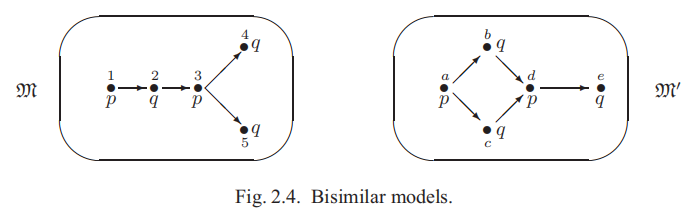
\includegraphics[width=.9\linewidth]{d:/media/wu/file/stuuudy/notes/images/ModalLogic/BisimilarModels.png}
\end{center}
\end{examplle}

\begin{examplle}[]
\label{example2.23}

\begin{center}
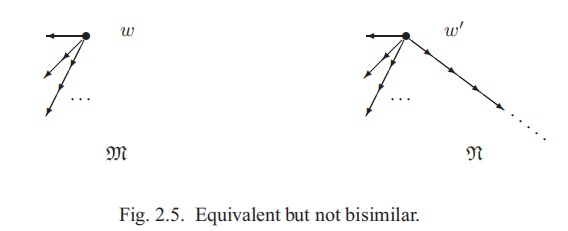
\includegraphics[width=.9\linewidth]{d:/media/wu/file/stuuudy/notes/images/ModalLogic/NotBisimilar.png}
\end{center}
\end{examplle}

\(\fM\) is \textbf{image-finite} if for each state \(u\) in \(\fM\) and each relation
\(R\) in \(\fM\), the set \(\{(v_1,\dots,v_n)\mid Ruv_1\dots v_n\}\) is
finite

\begin{theorem}[Hennessy-Milner Theorem]
\label{thm2.24}
Let \(\tau\) be a modal similarity type and let \(\fM\) and \(\fM'\) be two
image-finite \(\tau\)-models. Then for every \(w\in W\) and \(w'\in W'\),
\(w\leftrightarroweq w'\) iff \(w\leftrightsquigarrow w'\)
\end{theorem}

\begin{proof}
Assume that our similarity type \(\tau\) only contains a single diamond. The
direction from left to right follows from Theorem \ref{thm2.20}

Suppose \(w\leftrightsquigarrow w'\). The first condition is immediate. If
\(Rwv\), assume there is no \(v'\) in \(\fM'\) with \(R'w'v'\) and
\(v\leftrightsquigarrow v'\). Let \(S'=\{u'\mid R'w'u'\}\). Note that \(S'\)
must be non-empty, for otherwise \(\fM',w'\Vdash\Box\bot\), which would
contradict \(w\leftrightsquigarrow w'\) since \(\fM,w\Vdash\diamond\top\).
Furthermore, as \(\fM'\) is image-finite, \(S'\) must be finite, say
\(S'=\{w_1',\dots,w_n'\}\). By assumption, for every \(w_i'\in S'\) there
exists a formula \(\psi_i\) s.t. \(\fM,v\Vdash\psi_i\), but
\(\fM',w_i'\not\Vdash\psi_i\). It follows that
\begin{equation*}
\fM,w\Vdash\diamond(\psi_1\wedge\dots\wedge\psi_n)\quad\text{ and }\quad
\fM',w'\not\Vdash\diamond(\psi_1\wedge\dots\wedge \psi_n)
\end{equation*}
\end{proof}

\begin{exercise}
\label{ex2.2.8}
Suppose that \(\{Z_i\mid i\in I\}\) is a non-empty collection of
bisimulations between \(\fM\) and \(\fM'\). Prove that the relation
\(\bigcup_{i\in I}Z_i\) is also a bisimulation between \(\fM\) and \(\fM'\).
Conclude that if \(\fM\) and \(\fM'\) are bisimilar, then there is a maximal
bisimulation between \(\fM\) and \(\fM'\).
\end{exercise}

\begin{proof}
\begin{enumerate}
\item If \((w,w')\in\bigcup_{i\in I}Z_i\), then \((w,w')\in Z_j\) for some
\(j\in I\) and hence they satisfy the same propositional letters
\item If \((w,w')\in\bigcup_{i\in I}Z_i\) and \(R_{\triangle}wv_1\dots v_n\),
since \((w,w')\in Z_j\) for some \(j\in I\), we have
\(R'_{\triangle}w'v_1'\dots v_n'\) and \(v_iZ_jv_i'\) for all \(1\le i\le
      n\), which means \((v_i,v_i')\in\bigcup_{i\in I}Z_i\) for all \(1\le i\le n\)
\item similarly
\end{enumerate}
\end{proof}
\end{document}